\section{Auswertung}
\label{sec:Auswertung}

Die Maße, also Durchmesser $d$ bzw. Kantenlänge $a$ des eckigen Stabes mit quadratischem Querschnitt, Masse $m$ und Länge $l$ der Stäbe betragen

\begin{equation}
  a_{eckig} = 10,1 \pm 0,05mm \\
  m_{eckig} = 167,9 \pm 0,1g \\
  l_{eckig} = 620 \pm 0,05mm\\
\end{equation}

\begin{equation}
  d_{rund} = 10,1 \pm 0,05mm \\
  m_{rund} = 390,6 \pm 0,1g \\
  l_{rund} = 592 \pm 0,05mm \\
\end{equation}

Der eckige Stab besteht aus Aluminium, der runde aus Messing.\\
Um die Elastizitätsmodule zu bestimmen, müssen zuerst die Flächenträgheitsmomente $I$ nach --- errechnet werden.\\
Für den quadratischen Querschnitt mit Kantenlänge a ergibt sich die Formel $I_Q = \frac{a^4}{12}$ und 
für den kreisförmigen Querschnitt
$I_K = \frac{\pi r^4}{4}$. \\
Somit kommt man, die Gaußsche Fehlerfortpflanzung hinzugezogen, zu folgenden Flächenträgheitsmomenten:

\begin{equation}
  I_{rund} = \frac{\pi (0.5\cdot 10^{-3}m)^4}{4} = 4,91 \cdot 10^{-14}m^4 \quad 
  \textrm{und} \quad I_{eckig} = \frac{(1 \cdot 10^{-3}m)^4}{12} = 8,34 \cdot 10^{-14}m^4
\end{equation}

mit 

\begin{equation}
  \varDelta I_{rund} =  \sqrt{ (\frac{\partial I_{rund}}{\partial r})^2 \cdot (\varDelta r)^2} =  \\
  \textrm{und} \quad \varDelta I_{eckig} = \sqrt{ (\frac{\partial I_{eckig}}{\partial a})^2 \cdot (\varDelta a)^2} = 
\end{equation}

Damit berechnen sich die Elastizitätsmodule durch 

\begin{equation}
   E = \frac{F_g}{2 \cdot I \cdot a}   
\end{equation}

Mit $F = m \cdot 9.81 m/s^2$



\subsection{Einseitige Einspannung}
\label{sec:Einseitige Einspannung}

      \subsubsection{Runder Stab}
      \label{sec:Runder Stab}


\begin{table}[H]
  \centering
  \caption{Die Werte für die einseitige Einspannung bei Messung am runden Messingstab ohne Gewicht}
  \begin{tabular}{ccccc}
    \toprule
    {$x \mathbin{/} \unit{\milli\metre}$} &
    {$D_0(x) \mathbin{/} \unit{\milli\metre}$} \\
    \midrule
    34 & 0.01 \\  
    64 & 0.04 \\
    94 & 0.09 \\
    124 & 0.13 \\  
    154 & 0.19 \\
    184 & 0.22 \\
    214 & 0.26 \\
    244 & 0.33 \\
    274 & 1.03 \\
    304 & 1.05 \\
    334 & 1.07 \\
    364 & 1.28 \\
    394 & 1.25 \\
    424 & 1.30 \\
    454 & 1.32 \\
    484 & 1.38 \\

    \bottomrule
  \end{tabular}
  \label{tab:Tabelle3}
\end{table}



\begin{table}[H]
  \centering
  \caption{Die Werte für die einseitige Einspannung bei Messung am runden Messingstab mit einem Gewicht von 550g}
  \begin{tabular}{ccccc}
    \toprule
    {$x \mathbin{/} \unit{\milli\metre}$} &
    {$D_m(x) \mathbin{/} \unit{\milli\metre}$} \\
    \midrule
    25 & 0.25 \\
    55 & -0.07 \\
    85 & -0.09 \\
    115 & -0.07 \\
    145 & -0.01 \\
    175 & 0.12 \\
    205 & 0.26 \\ 
    235 & 0.46 \\
    265 & 0.73 \\
    295 & 1.00\\
    325 & 1.31 \\
    355 & 1.62 \\
    385 & 2.00 \\
    415 & 2.39 \\
    445 & 2.75 \\
    475 & 3.37 \\
    497 & 3.54 \\
    
    \bottomrule
  \end{tabular}
  \label{tab:Tabelle3}
\end{table}

Zur Ermittlung des Elastizitätsmodul wird eine lineare Regression durchgeführt, wobei $D(x) = D_m - D_0$ gegen 
$Lx^2 - \frac{x^3}{3}$ aufgetragen wird.\\
So werden die folgenden Werte der Steigung a der Ausgleichsgeraden und des y-Achsenabschnitts c ermittelt:

% fehlt noch, außerdem wieder E berechnen mit folgender glecihung

\begin{equation}
  E = \frac{m \cdot 9.81 m/s^2}{2 \cdot I \cdot a} %hier rechnung einfügen, a ist die steigung, nicht kantenlänge
\end{equation}
 


\begin{figure}
  \centering
  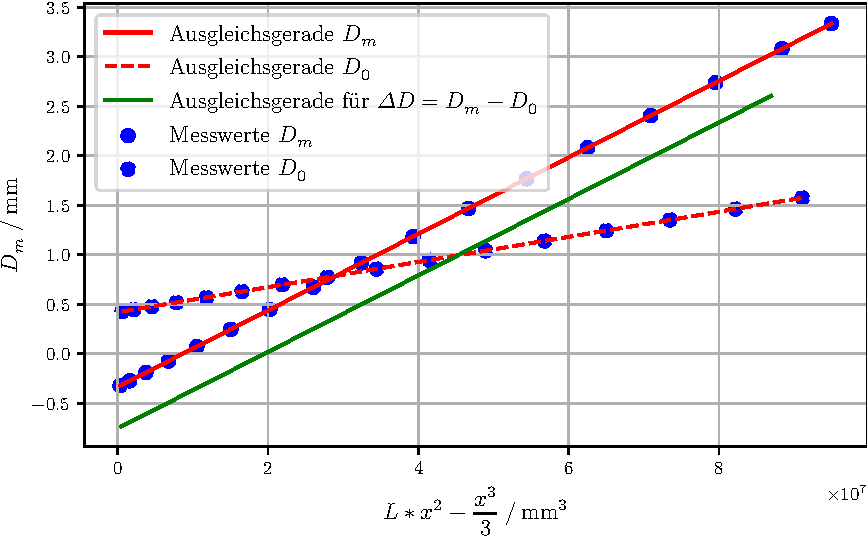
\includegraphics{plot_messing_einseitig.pdf}
  \caption{Plot.}
  \label{fig:plot}
\end{figure}

\subsubsection{Eckiger Stab}
\label{sec:Eckiger Stab}

\begin{table}[H]
  \centering
  \caption{Die Werte für die einseitige Einspannung bei Messung am eckigen Aluminiumstab ohne Gewicht}
  \begin{tabular}{ccccc}
    \toprule
    {$x \mathbin{/} \unit{\milli\metre}$} &
    {$D_0(x) \mathbin{/} \unit{\milli\metre}$} \\
    \midrule
    25 & 0.00 \\
    55 & -0.08 \\
    85 & -0.15 \\
    115 & -0.22 \\
    145 & -0.29 \\
    175 & -0.33 \\   
    205 & -0.38 \\
    235 & -0.41 \\
    275 & -0.44 \\
    305 & -0.40 \\
    335 & -0.44 \\
    365 & -0.43 \\
    395 & -0.43 \\
    425 & -0.43 \\
    
    \bottomrule
  \end{tabular}
  \label{tab:Tabelle3}
\end{table}

\begin{table}[H]
  \centering
  \caption{Die Werte für die einseitige Einspannung bei Messung am eckigen Aluminiumstab mit einem Gewicht von 550g}
  \begin{tabular}{ccccc}
    \toprule
    {$x \mathbin{/} \unit{\milli\metre}$} &
    {$D_m(x) \mathbin{/} \unit{\milli\metre}$} \\
    \midrule
    25 & 0.05 \\
    55 & 0.29 \\
    85 & 0.58 \\
    115 & 0.94 \\
    145 & 1.30 \\ 
    175 & 1.75 \\
    205 & 2.20 \\    
    235 & 2.74 \\
    265 & 3.24 \\
    295 & 3.81 \\
    325 & 4.40 \\
    355 & 5.05 \\
    385 & 5.65 \\
    415 & 6.25 \\
    
    \bottomrule
  \end{tabular}
  \label{tab:Tabelle3}
\end{table}

Analog zum runden Messingstab lässt sich auch das Elastizitätsmodul des eckigen Stabes aus Aluminium bestimmen.\\
Steigung und y-Achsenabschnitt lauten:      % einfügen

Somit ergibt sich für $E_{eckig}$ daraus:

\begin{equation}
  E_{eckig} =             % einfügen
\end{equation}


\begin{figure}
  \centering
  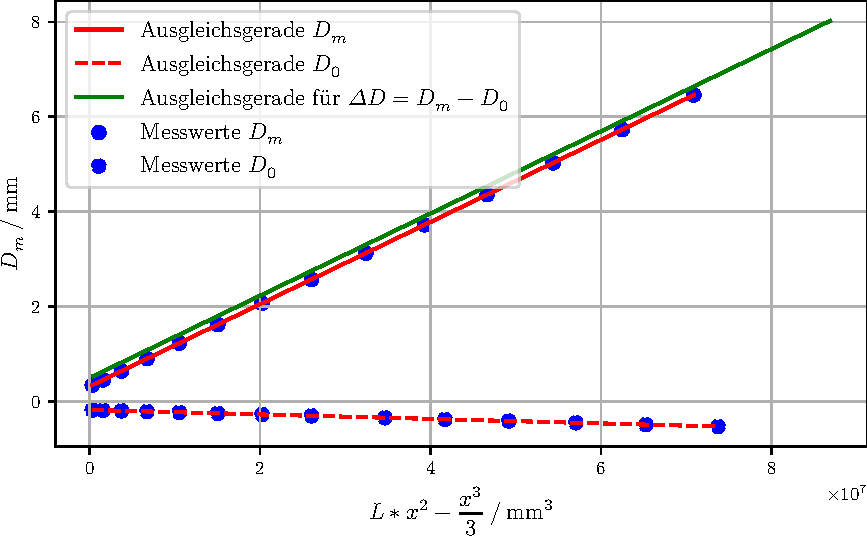
\includegraphics{plot_alu_einseitig.pdf}
  \caption{Plot.}
  \label{fig:plot_alu_einseitig}
\end{figure}




\subsection{Beidseitige Auflage}
\label{sec:Beidseitige Auflage}



\begin{table}[H]
  \centering
  \caption{Die Werte für die beidseitige Auflage bei Messung am runden Messingstab von rechts bis zur Mitte, bei $D_m$ mit 
  einem Gewicht von 1250g}
  \begin{tabular}{ccccc}
    \toprule
    {$x \mathbin{/} \unit{\milli\metre}$} &
    {$D_0(x) \mathbin{/} \unit{\milli\metre}$} &
    {$D_m(x) \mathbin{/} \unit{\milli\metre}$} \\
    \midrule
    30 & 0.01 & 0.20  \\  
    60 & 0.04 & 0.48 \\
    90 & 0.09 & 0.71 \\
    120 & 0.13 & 0.93 \\
    150 & 0.19 & 1.14 \\
    180 & 0.22 & 1.32 \\
    210 & 0.26  & 1.46 \\
    240 & 0.33 & 1.58 \\
    
    \bottomrule
  \end{tabular}
  \label{tab:Tabelle3}
\end{table}



\begin{table}[H]
  \centering
  \caption{Die Werte für die beidseitige Auflage bei Messung am runden Messingstab von rechts bis zur Mitte, bei $D_m$ mit 
  einem Gewicht von 1250g}
  \begin{tabular}{ccccc}
    \toprule
    {$x \mathbin{/} \unit{\milli\metre}$} &
    {$D_0(x) \mathbin{/} \unit{\milli\metre}$} &
    {$D_m(x) \mathbin{/} \unit{\milli\metre}$} \\
    \midrule
    0 & 0.00 & 0.10
    30 & 0.09 & 0.20  \\  
    60 & 0.15 & 0.32 \\
    90 & 0.24 & 0.41 \\
    120 & 0.32 & 0.50 \\
    150 & 0.35 & 0.58 \\
    180 & 0.42 & 0.65 \\
    210 & 0.45 & 0.70 \\
    240 & 0.52 & 0.71 \\
    \bottomrule
  \end{tabular}
  \label{tab:Tabelle3}
\end{table}


Die Werte für die beidseitige Auflage werden für die lineare Regression in D(x) gegen $3L^2 x - 4x^3$ aufgetragen.

Mit den sich ergebenden Werten für $a$ und $c$ lässt sich $E = \frac{m \cdot g}{48 \cdot I \cdot a}$ mit wie folgt berechnen



\begin{figure}
  \centering
  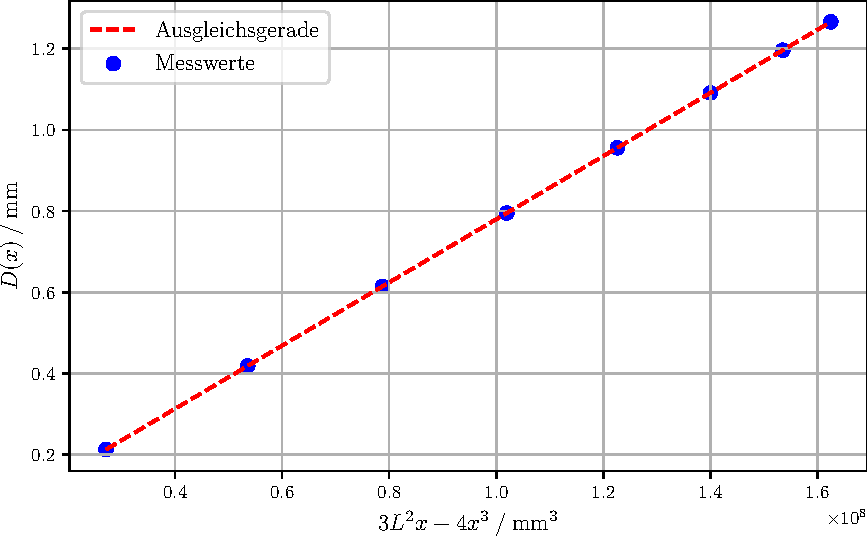
\includegraphics{plot_beidseitig_rechts.pdf}
  \caption{Die lineare Regression für die Messung am beidseitig aufliegenden, runden Messingstab von rechts}
  \label{fig:plot_beidseitig_rechts}
\end{figure} 

\begin{figure}
  \centering
  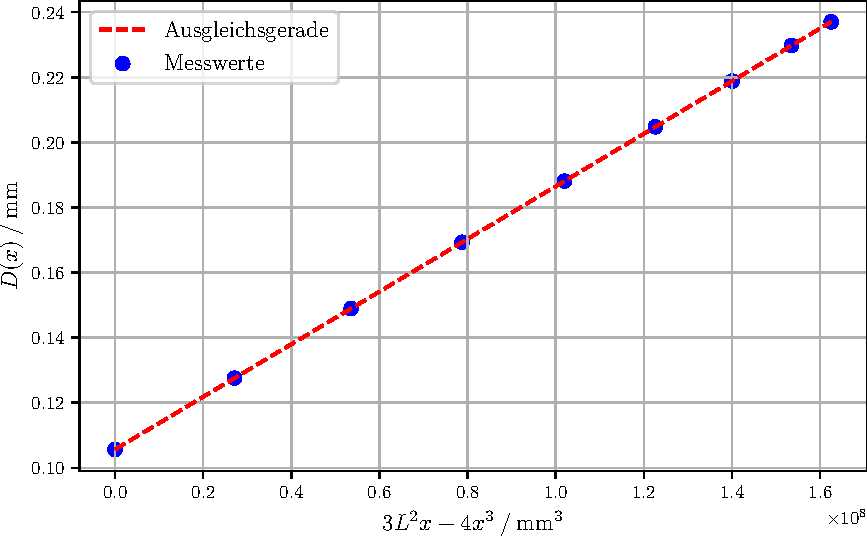
\includegraphics{plot_beidseitig_links.pdf}
  \caption{Die lineare Regression für die Messung am beidseitig aufliegenden, runden Messingstab von links}
  \label{fig:plot_beidseitig_links}
\end{figure}       % irgendwie ist die achsenbeschriftung bei diesen beiden plots ncoh falsch, obwohl sie in der 
                   % plot.py schon richtig ist. sollte 3L^2 x - 4x^3 statt Lx^2...


Siehe \autoref{fig:plot}! 
